\begin{pastexam}[label={px:gw3-096-ds-04}]{關務三等資訊處理 96 年 第四題}
（申論；15 分）

費氏級數定義於下：
\[
\mathrm{F}(\mathrm{N}) = \begin{cases} \mathrm{F}(\mathrm{N} - 1) + \mathrm{F}(\mathrm{N} - 2)\,, & \text{if } \mathrm{N} \ge 2 \\
1\,, & \text{if } \mathrm{N} = 1 \\ 0\,, & \text{if } \mathrm{N} = 0 \end{cases}
\]
\begin{itemize}[leftmargin=2.2em, nosep]
\item[㈠] 試求算 F(5) 的值。（5 分）
\item[㈡] 計算 F(5) 的值需呼叫函數的次數。（5 分）
\item[㈢] 計算 F(5) 的值需加法運算的次數。（5 分）
\end{itemize}
\end{pastexam}

\begin{pastsoln}
答案：㈠ $5$。 ㈡ $15$ 次。 ㈢ $7$ 次。

題目沒有說用哪種方法算，㈡㈢ 問呼叫次數，表示是照定義直接寫成遞迴函式來算（每次呼叫 F 都算一次，包括最外層的
$\mathrm{F}(5)$）。

\textbf{㈠} 由下往上：$\mathrm{F}(2) = 1$，$\mathrm{F}(3) = 2$，$\mathrm{F}(4) = 3$，$\mathrm{F}(5) = 5$。

\textbf{㈡ 呼叫次數。} 設 $C(n)$ 是計算 $\mathrm{F}(n)$ 總共的呼叫次數（含自己這一次）。 $n \le 1$ 時直接傳回，$C(0) = C(1) = 1$；
$n \ge 2$ 時自己一次加上兩個子呼叫：
\[
C(n) = 1 + C(n - 1) + C(n - 2).
\]
所以 $C(2) = 3$，$C(3) = 5$，$C(4) = 9$，$C(5) = 1 + 9 + 5 = 15$。 遞迴樹畫出來就是 $15$ 個節點：
\begin{center}
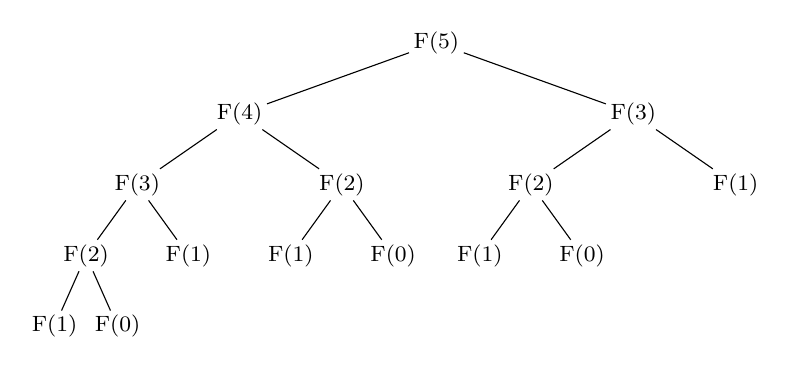
\begin{tikzpicture}[every node/.style={inner sep=1.5pt,font=\footnotesize},
  level distance=9mm, level 1/.style={sibling distance=50mm}, level 2/.style={sibling distance=26mm},
  level 3/.style={sibling distance=13mm}, level 4/.style={sibling distance=8mm}]
\node {F(5)}
  child {node {F(4)}
    child {node {F(3)} child {node {F(2)} child {node {F(1)}} child {node {F(0)}}} child {node {F(1)}}}
    child {node {F(2)} child {node {F(1)}} child {node {F(0)}}}}
  child {node {F(3)}
    child {node {F(2)} child {node {F(1)}} child {node {F(0)}}}
    child {node {F(1)}}};
\end{tikzpicture}
\end{center}

\textbf{㈢ 加法次數。} 每個 $n \ge 2$ 的呼叫做一次加法，$n \le 1$ 的不做。 設 $A(n)$ 是加法次數，$A(0) = A(1) = 0$，
\[
A(n) = 1 + A(n - 1) + A(n - 2),
\]
得 $A(2) = 1$，$A(3) = 2$，$A(4) = 4$，$A(5) = 7$。 從樹上看：$15$ 個節點中 $8$ 個是葉子（F(1) 或 F(0)），$7$ 個內部節點
各做一次加法。 一般而言 $C(n) = 2\mathrm{F}(n + 1) - 1$、$A(n) = \mathrm{F}(n + 1) - 1$，都隨 $n$ 指數成長，因為同一個
$\mathrm{F}(k)$ 被重複算了很多次（上圖 $\mathrm{F}(2)$ 就算了三次）。 改用由下往上的迴圈或把算過的值記起來
（資結書第~18.1~節），只要 $n - 1 = 4$ 次加法。
\end{pastsoln}
